\subsection{Configuration and Logging}
ANT, Visual Studio Project Files, Java Logging Framework, ...
\subsection{Webservices}
Eine exakte Definition gibt es nicht. Einige würden sogar den Aufruf auf eine einfache Website als Webservice bezeichnen. Grundsätzlich lässt sich aber sagen, dass ein Webservice sowohl einen Request akzeptiert und eine Response generiert oder zumindest einen Task ausführt. Zumindest lässt sich sagen, dass der Request oder die Response aus XML besteht.

\subsection{Unterschied RPC und SOAP}
Bei RPC sehen weder Nutzer noch Service je XML (XML wird nur für Transport verwendet).
\begin{figure}[h!]
\centering
\small
\begin{tikzpicture}[->, >=stealth', auto, semithick, node distance=2cm]
\tikzstyle{every state}=[fill=white,draw=black,thick,text=black,scale=1]
\fill [blue!20] (-4,0.5) rectangle (11.5,2.5);
\node (rect)    (C) at (4,4) [draw,thick] {Client};
\node (rect)    (S) at (2,4) [draw,thick] {Server};
\node (rect)    (M) at (3,2) [draw,thick] {Middleware};
\node[blue] at (8,1) {XML};
\path
(C) edge[left,right] node{1. Methodenaufruf mit Parametern} (M)
(M) edge[loop right] node{2. Verpacken des Aufrufs in XML File} (M)
(M)	edge[loop below] node{3. Senden zur Middleware des Servers}(M)
(M)	edge[loop left] node{4. Entpacken des XML Files}(M)
(M) edge[left,left] node{5. Methodenaufruf auf Server mit Parametern} (S);
\end{tikzpicture}
\caption{RPC Aufruf Client $\rightarrow$ Server}
\end{figure}
\\
In Listing \ref{lst:webservicerequest} ist dargestellt, wie ein Aufruf der Methode \code{MathService.Add(17,29)} in der Middleware zu einem XML verarbeitet werden könnte. Die Response des Servers könnte dazu wie in Listing \ref{lst:webserviceresponse} dargestellt aussehen.\\
\begin{minipage}{0.45\textwidth}
\begin{lstlisting}[language=XML, caption={Web Service Request}, label=lst:webservicerequest]
<methodCall> 
<methodName>MathService.Add</methodName> 
<params>
    <param>
      <value>
        <double>17</double>
      </value>
    </param>
    <param>
	 <value> 
		<double>29</double>
      </value>
    </param>
  </params>
</methodCall>
\end{lstlisting}
\end{minipage}
\hfill
\begin{minipage}{0.45\textwidth}
\begin{lstlisting}[language=XML, caption={Web Service Response}, label=lst:webserviceresponse]
<methodResponse>
  <params>
	<param>
	 <value>
        <double>46</double>
      </value>
    </param>
  </params>
</methodResponse>
\end{lstlisting}
\end{minipage}\\
Bei SOAP haben User und Service Zugriff auf ein XML File. Eine SOAP-Message hat einen sogenannten \code{<envelope>}-Tag, das einen \code{<header>} und einen \code{<body>} enthält. Der Header enthält Informationen über den Request, der Body enthält eine XML Node	. SOAP arbeitet gut mit XML-Encryption und Signaturen zusammen.\\
\begin{minipage}{0.45\textwidth}
\begin{lstlisting}[language=XML, caption={SOAP-Envelope}, label=lst:soapenvelope]
<soap:Envelope
xmlns:soap="http://www.w3.org/2003/05/soap-envelope/"
soap:encodingStyle="http://www.w3.org/2003/05/soap-encoding">

<soap:Header>
  <m:Trans xmlns:m="http://www.w3schools.com/transaction/"
  soap:mustUnderstand="1">234
  </m:Trans>
</soap:Header>

<soap:Body>
  <m:GetPrice xmlns:m="http://www.w3schools.com/prices">
    <m:Item>Apples</m:Item>
  </m:GetPrice>
</soap:Body>
</soap:Envelope>
\end{lstlisting}
\end{minipage}
\hfill
\begin{minipage}{0.45\textwidth}
\begin{lstlisting}[language=XML, caption={Extracted Message}, label=lst:soapextractedmessage] 
<GetPrice xmlns:m="http://www.w3schools.com/prices">
  <Item>Apples<Item>
 </GetPrice>
\end{lstlisting}
\end{minipage}\\

\subsection{Web Service Description Language (WSDL)}
\begin{minipage}{0.6\textwidth}
SOAP transportiert jede XML-Node, aber wie können wir wissen, wie ein SOAP-Request auszusehen hat? Dieses Problem wird durch die WSDL (eine XML-Sprache) durch zur Verfügung stellen eines Contracts zwischen dem Webservice und der Aussenwelt gelöst. Ein solcher Contract definiert, welches Format der Server erwartet und ebnenso, wie die Antwort des Servers dazu aussieht. Dafür gibt es mittlerweile Tools, der Informatiker muss sich also nicht mehr direkt mit WSDL-Dokumenten auseinandersetzen.
\end{minipage}
\hfill
\begin{minipage}{0.4\textwidth}
\centering
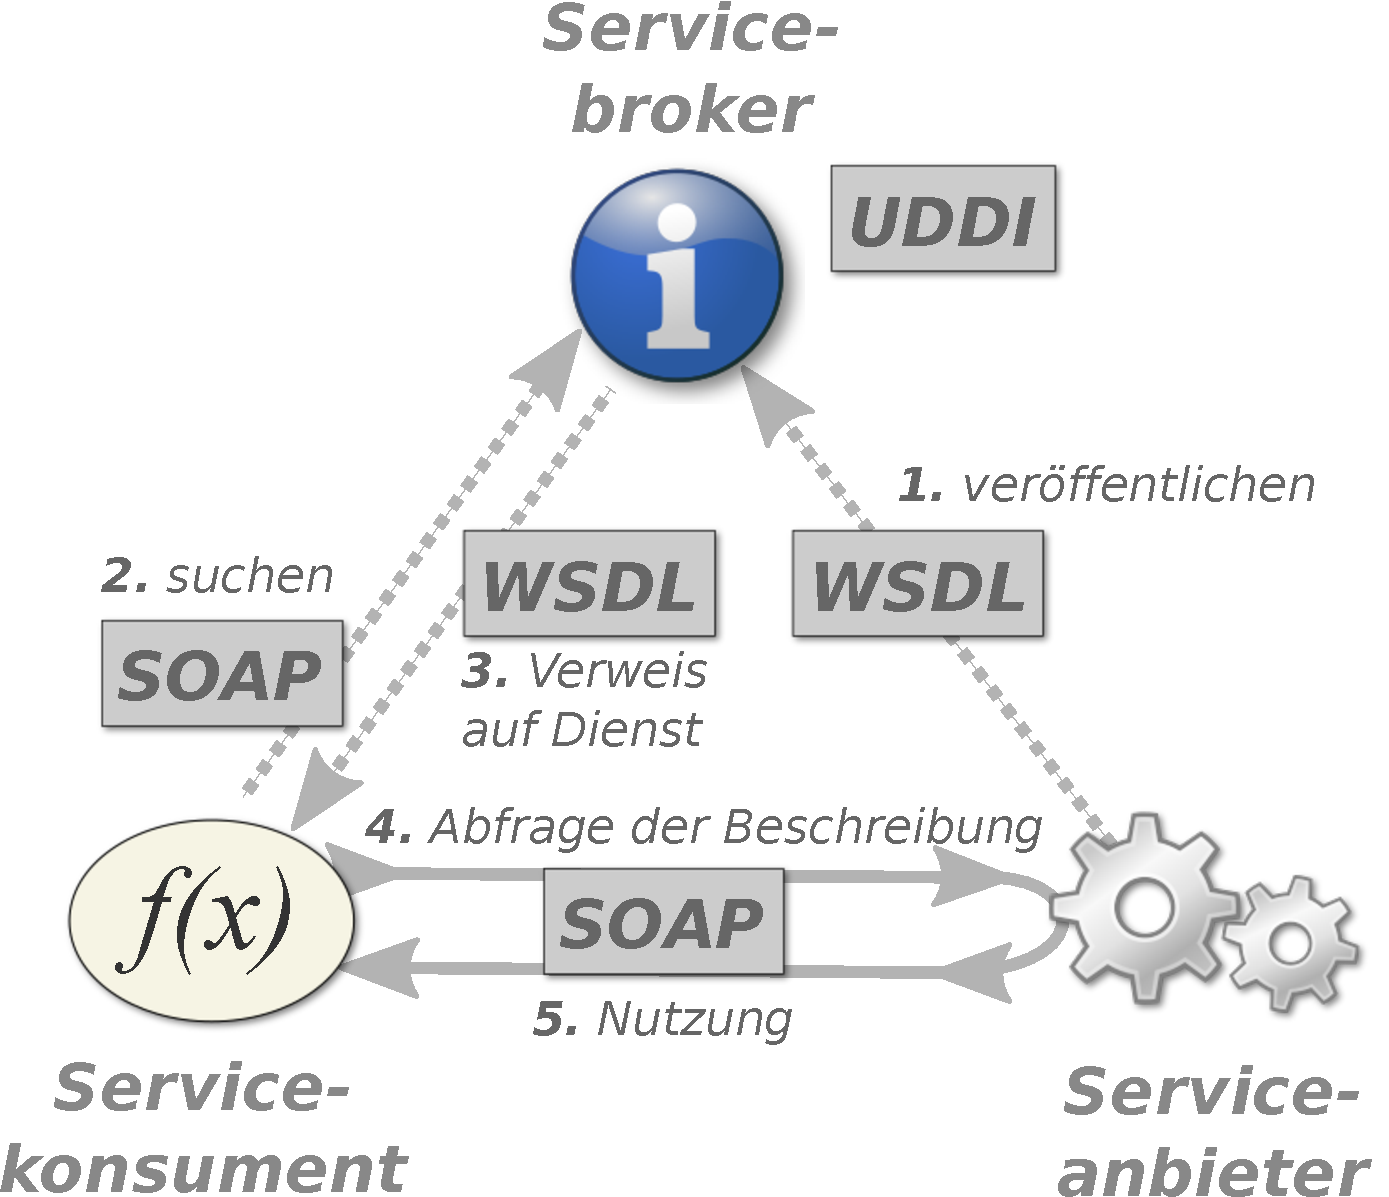
\includegraphics[width=\textwidth]{fig/Webservice.pdf}
\captionof{figure}{WSDL}
\end{minipage}\\
\subsection{UDDI - How to find Web Services in  the Wild}
Das Universal Discovery, Description and Integration (UDDI) erlaubt es, Webservices zu registrieren, damit diese von Programmierern und anderen Webservices gefunden werden können.
Das global UDDI Registry besteht aus mehreren Servern, die sich alle spiegeln: Register once, find everywhere!
Mit dem Webservice registriert man auch seine Kontaktinformationen. Eine andere Firma kann UDDI nutezn, um Businesspartner zu finden, die Dienste anbietet, die sie benötigt.

\subsection{Web Content and Type Setting}
XHTML, MATHML, SVG

\subsection{Business Interoperability}
\begin{figure}[h!]
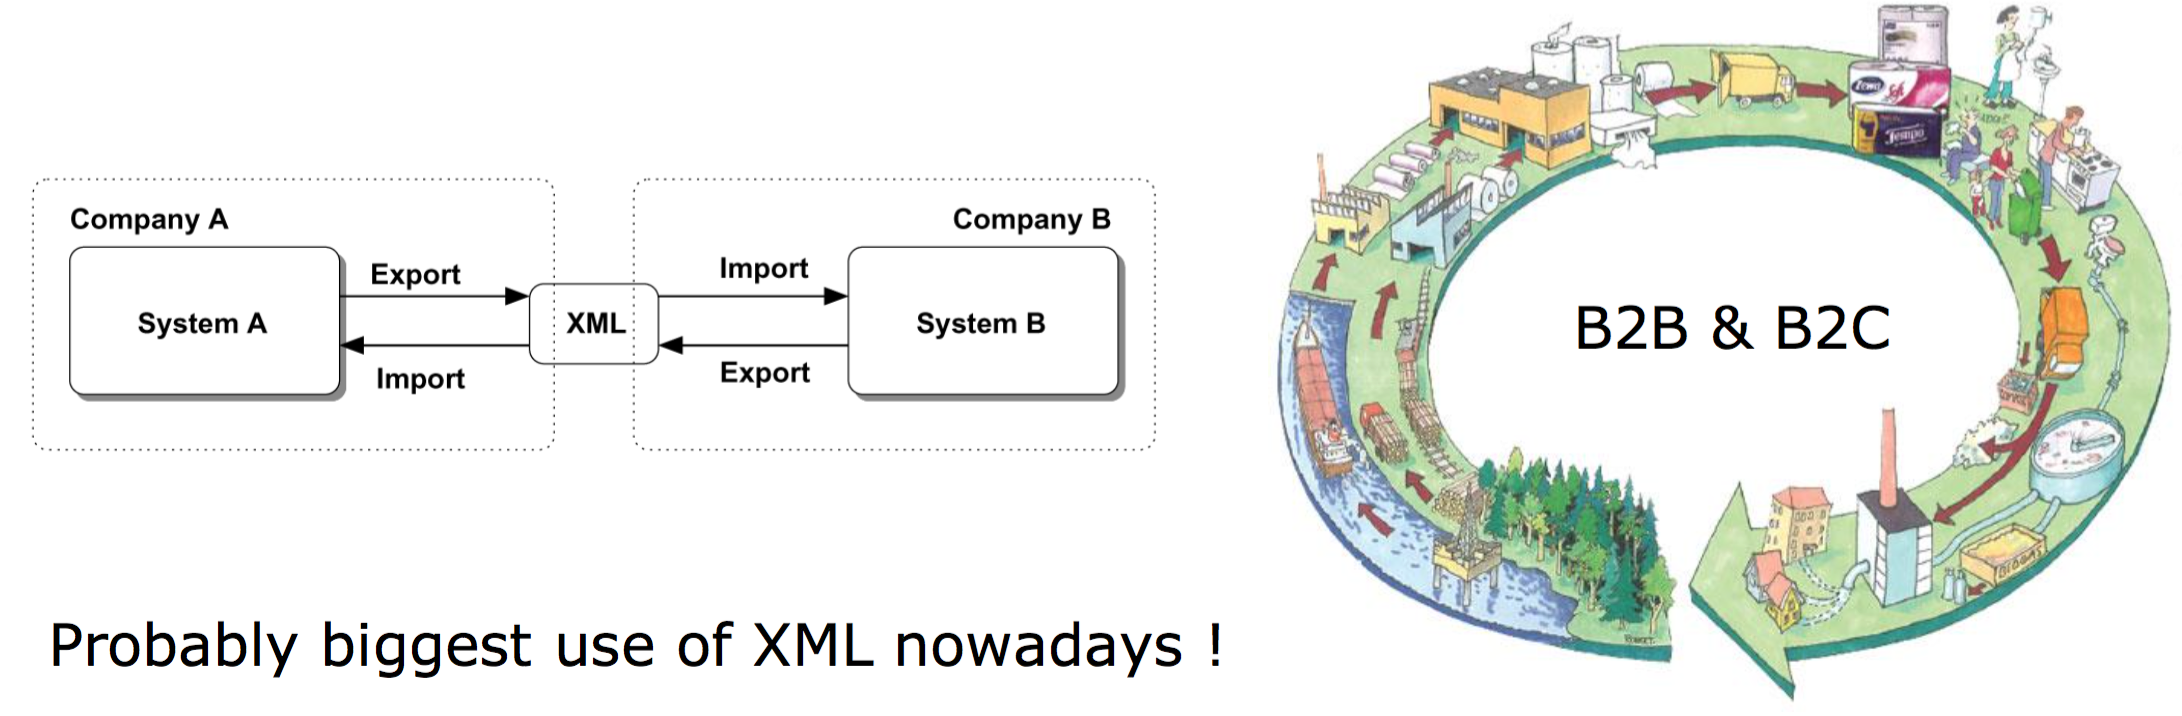
\includegraphics[width=\textwidth]{fig/Businessinteroperability.png}
\end{figure}

\subsection{Data Carrier}
Weiter in Kapitel 9